\chapter{Aplicații ale aritmeticii modulare}
\label{sec:apl-mod}

Cel mai rapid algoritm al lui Euclid lucrează modulo 2.

\begin{algorithm}
  \caption{Euclid modulo 2}
  \label{alg:euclid-2}
  \begin{algorithmic}[1]
    \Procedure{Euclid mod 2}{a,b}
    \State $ g \gets 1 $
    \While{$(a \% 2 = 0 \&\& b \% 2 = 0)$}
    \State $ a \gets a/2 $
    \State $ b \gets b/2 $
    \State $ g \gets 2g $
    \EndWhile
    \While{$(a \neq 0)$}
    \While{$(a \% 2 = 0)$} \State $ a \gets a/2 $ \EndWhile
    \While{$(b \% 2 = 0)$} \State $ b \gets b/2 $ \EndWhile
    \Comment{acum ambii sînt impari}
    \If{$(a \geq b)$} $ a \gets (a-b)/2 $
    \Else $ b \gets (b - a)/2 $
    \EndIf
    \EndWhile
    \Return $ g \cdot b $
    \EndProcedure
  \end{algorithmic}
\end{algorithm}

O variantă optimizată putem formula și pentru lema chineză a resturilor și
obținem \emph{varianta efectivă}, adică: presupunem că avem $ m_1, \dots, m_r $
astfel încît $ \forall i \neq j, \dr{gcd}(m_i, m_j) = 1 $. Vrem să găsim $ x $
astfel încît pentru orice $ i $, $ x = a_i \text{ mod } m_i $.

Fie $ M = m_1 \cdots m_r $ și $ M_i = \dfrac{M}{m_i} $. Definim
$ y_i = M_i^{-1} \text{ mod } m_i $. Atunci soluția este:
\[
  x = \sum_{i = 1}^r a_i M_i y_i \text{ mod } M.
\]

De exemplu: căutăm $ x $ astfel încît:
\begin{align*}
  x &= 5 \text{ mod } 7 \\
  x &= 3 \text{ mod } 11 \\
  x &= 10 \text{ mod } 13.
\end{align*}

Fie $ M = 7 \cdot 11 \cdot 13 = 1001 $. Atunci:
\begin{align*}
  M_1 &= 11 \cdot 13 = 143, \quad y_1 = 143^{-1} \text{ mod } 7 = 3^{-1} \text{ mod } 7 = 5 \\
  M_2 &= 7 \cdot 13 = 91, \quad y_2 = 91^{-1} \text{ mod } 11 = 3^{-1} \text{ mod } 11 = 4 \\
  M_3 &= 7 \cdot 11 = 77, \quad y_3 = 77^{-1} \text{ mod } 13 = 12^{-1} \text{ mod } 13 = 12.
\end{align*}

Rezultă:
\[
  x = \sum a_i M_i y_i \text{ mod } M = 894 \text{ mod } 1001.
\]

Obținem de aici că în izomorfismul $ \ZZ_{1001} \simeq \ZZ_7 \times \ZZ_{11} \times \ZZ_{13} $,
894 corespunde tripletului $(5, 3, 10) $.

%%%%%%%%%%%%%%%%%%%%%%%%%%%%%%%%%%%%%%%%%%%%%%%%%%%%%%%%%%%%%%%%%%%%%%

\section{Coduri liniare}

Fie $ \kal{A} $ un alfabet, cu $ \# A = n $. Putem identifica $ \kal{A} $ cu $ \ZZ_n $
și atunci o aplicație $ C : \kal{A}^k \to \kal{A}^k $ este dată de:
\[
  C(a_1, \dots, a_k) = M \cdot (a_1 \ \dots \ a_k)^t,
\]
unde $ M \in M_k(\ZZ_n) $ este o matrice inversabilă.

Amintim că, în general, dacă $ M \in M_k(R) $, cu $ R $ un inel oarecare,
avem că $ M $ este inversabilă dacă și numai dacă $ \det(M) \in R^\times $.

De exemplu, să luăm $ \kal{A} $ alfabetul latin cu 26 de litere și
aplicăm codarea $ x_1 x_2 \leadsto y_1 y_2 $, conform ecuațiilor:
\[
  \begin{cases}
    y_1 &= 6x_1 + 2x_2 \text{ mod } 26 \\
    y_2 &= 5x_1 + 2x_2 \text{ mod } 26.
  \end{cases}
\]

Căutăm cuvinte $ x_1 x_2 $ și $ x_1'x_2' $ care au aceeași codificare
$ y_1 y_2 $. Dacă acestea există, atunci această codificare nu poate
fi folosită în criptografie, din cauza ambiguităților introduse!

Rezolvarea problemei revine la rezolvarea sistemului de congruențe,
folosind matricea sistemului:
\[
  A = %
  \begin{pmatrix}
    6 & 1 \\
    5 & 1
  \end{pmatrix} \text{ mod } 26.
\]
Cum $ \det(A) = 1 $, matricea este inversabilă, deci sistemul are soluție unică.

Regula de decriptare este dată de înmulțirea la dreapta a formei matriceale
a sistemului cu $ A^{-1} $.

%%%%%%%%%%%%%%%%%%%%%%%%%%%%%%%%%%%%%%%%%%%%%%%%%%%%%%%%%%%%%%%%%%%%%%

\section{Securitate bazată pe teoria informației}

Fie $ P $ mulțimea textelor clare (\emph{plain text}), $ K $,
mulțimea cheilor și $ C $, mulțimea textelor codificate.
Atunci avem funcțiile care ne dau criptarea și decriptarea:
\begin{itemize} \index{criptare!simetrică}
\item $ \dr{Enc} : P \times K \to C $;
\item $ \dr{Dec} : C \times K \to P, \dr{Dec}_k(\dr{Enc}_k(m)) = m $,
  adică are loc o \emph{criptare simetrică}.
\end{itemize}

\begin{definition}\label{def:sec-perf} \index{securitate!perfectă}
  Spunem că sistemul $ (\dr{Enc}, \dr{Dec}) $ \emph{are securitate perfectă}
  dacă și numai dacă, $ \forall m \in P, \forall c \in C, p(m \mid c) = p(m) $,
  unde $ p $ este probabilitatea.

  Cu alte cuvinte, chiar dacă îl știm pe $ c $, nu avem nicio informație despre $ m $.
\end{definition}

Din proprietăți elementare ale funcțiilor, avem:
\begin{lemma}\label{le:sec-perf}
  Dacă securitatea este perfectă, atunci $ \# K \geq \# C \geq \# P $.
\end{lemma}

\begin{proof}
  Se poate vedea că $ \dr{Enc}_k $ este injectivă, pentru orice cheie fixată
  $ k \in K $, deci $ \# C \geq \# P $.

  Acum, pentru orice $ c \in C, p(c) > 0 $ (altfel, $ c $ este inutilă).
  Rezultă că pentru orice $ m \in P, c \in C $, $ p(c | m) = p(c) > 0 $\footnotemark.
  Atunci, pentru orice mesaj $ m \in P $ și orice codificare $ c \in C $, există
  o cheie $ k \in K $ cu $ \dr{Enc}_k(m) = c $. De aici, $ \# K \geq \# C $.
\end{proof}

\footnotetext{Am folosit \emph{formula probabilităților condiționate}:
  \[
    P(A | B) = \dfrac{P(A \cap B)}{P(B)}.
  \]
  \index{probabilități!condiționate}
}

\begin{theorem}[Shannon]\label{thm:shannon}
  \index{teoremă!Shannon}
  Dacă $ \# P = \# C = \# K $, atunci securitatea perfectă este echivalentă
  cu afirmațiile:
  \begin{itemize}
  \item orice cheie este folosită cu probabilitate egală, $ \dfrac{1}{\# K} $;
  \item pentru orice mesaj $ m \in P $ și codare $ c \in C $, există o cheie
    unică $ k \in K $, cu $ \dr{Enc}_k(m) = c $.
  \end{itemize}
\end{theorem}

\begin{proof}
  \qq{$\Longrightarrow$}: Trebuie să arătăm că pentru orice mesaj $ m $ din $ P $,
  există o cheie unică pentru descifrare. Cum $ \# C = \# K $, rezultă:
  \[
    \# \{ \dr{Enc}_k(m) \mid k \in K \} = \# K
  \]
  și avem concluzia.

  Vrem să arătăm că fiecare cheie este folosită cu probabilitate egală,
  anume $ p(k) = \dfrac{1}{\# K} $, pentru orice $ k \in K $.

  Fie $ \# K = n, P = \{ m_i \mid 1 \leq i \leq n \} $ și fie $ c \in C $ fixat.
  Indexăm cheile $ k_1, \dots, k_n $ astfel încît $ \dr{Enc}_{k_i}(m_i) = c, \forall i $.

  Securitatea perfectă ne asigură că $ p(m_i \mid c) = p(m_i) $, deci:
  \[
    p(m_i) = p(m_i \mid c) = \frac{p(c\mid m_i) p(m_i)}{p(c)} = %
    \frac{p(k_i)p(m_i)}{p(c)}.
  \]
  Rezultă că pentru orice $ i $, avem $ p(k_i) = p(c) $, adică toate cheile
  au probabilitate egală și ea este $ \dfrac{1}{n} $.

  \qq{$\Longleftarrow$} Reciproc, știind că $ \# K = \# P = \# C $ și
  $ p(k) = \dfrac{1}{\# K}, \forall k \in K $ și că pentru orice mesaj
  există o cheie unică de descifrare, arătăm că $ p(m \mid c) = p(m) $.

  Calculăm:
  \[
    p(c) = \sum_{k \in K} p(k) p(m = \dr{Dec}_k(c)) = %
    \frac{1}{\# K} \sum_k p(m = \dr{Dec}_k(c))
  \]
egalitatea avînd loc deoarece cheile au probabilitate egală.

Deoarece pentru orice mesaj $ m $ și criptare $ c $, există o
cheie unică $ k $, cu $ \dr{Enc}_k(m) = c $, rezultă:
\[
  \sum_{k \in K} p(m = \dr{Dec}_k(c)) = \sum_m p(m) = 1,
\]
adică, încercînd toate cheile, sigur descifrăm mesajul.
Rezultă $ p(c) = \dfrac{1}{\# K} $. Iar dacă $ c = \dr{Enc}_k(m) $,
atunci $ p(c \mid m) = p(k) = \dfrac{1}{\# K} $.

Folosim teorema lui Bayes:
\begin{theorem}[Bayes]\label{thm:bayes}
  \index{probabilități!teorema Bayes}
  Fie $ X $ și $ Y $ două variabile aleatoare, cu $ p(Y = y) > 0 $. Atunci:
  \[
    p(X = x \mid Y = y) = \frac{p(X = x) \cdot p(Y = y \mid X = x)}{p(Y = y)}.
  \]
\end{theorem}

Se obține:
\[
  p(m | c) = \dfrac{p(m) \cdot p(c \mid m)}{p(c)} = \dfrac{p(m) \cdot \dfrac{1}{\# K}}{%
    \dfrac{1}{\# K}} = p(m),
\]
ceea ce finalizează demonstrația.
\end{proof}


\begin{example}
  Fie $ \kal{A} = \{ A, B, \dots, Z \} $ alfabetul cu 26 de litere.

  Atunci $ \# K = \# P = \# C = 26^n $, iar $ p(k) = \dfrac{1}{26^n} $.

  Criptarea se face prin $ c = m + k \text{ mod } 26 $, pe componente.
\end{example}

\begin{example}
  \textbf{Vernam's Code (OTP)}: Fie $ \# K = \# P = \# C = 2^n $,
  iar $ p(k) = 2^{-n} $. Atunci criptarea se face prin $ c = m \oplus k $,
  unde $ \oplus $ este adunarea binară (i.e.\ suma pe $ \FF_2 = \ZZ_2 $).

  Atenție, însă: dacă se folosește aceeași cheie, întrucît:
  \[
    c_1 \oplus c_2 = m_1 \oplus k \oplus m_2 \oplus k = m_1 \oplus m_2,
  \]
  se poate face analiză de frecvența, iar mesajul poate fi descifrat.
\end{example}

\section{Entropia}

\begin{definition}\label{def:entropie}
  \index{probabilități!entropie}
  Fie $ X $ o variabilă aleatoare, care ia valorile $ x_1, \dots, x_n $, cu
  probabilitățile $ p_i = p(X = x_i) $.

  Se definește \emph{entropia} variabilei aleatoare prin:
  \[
    H(X) = - \sum_{i = 1}^n p_i \log_2 p_i,
  \]
  cu convenția că dacă $ p_i = 0 $, atunci $ p_i \log_2 p_i = 0 $.
\end{definition}

De exemplu, dacă la o întrebare răspund mereu \qq{da}, atunci $ p_1 = 1, p_2 = 0 $.

Entropia este $ H(X) = -1 \log_2 1 - 0 \log_2 0 = 0 $, adică nu ofer nicio informație.

Dacă răspund la întîmplare cu \qq{da} sau \qq{nu}, atunci $ p_1 = p_2 = \dfrac{1}{2} $
și:
\[
  H(X) = \frac{1}{2} \cdot \Big( -\log_2 \frac{1}{2} - \log_2 \frac{1}{2} \Big) = 1,
\]
adică ofer 1 bit de informație.

Se poate vedea că funcția entropie are proprietățile:
\begin{itemize}
\item $ H(X) \geq 0 $, pentru orice variabilă aleatoare;
\item $ H(X) = 0 $ dacă și numai dacă există un singur eveniment sigur,
  iar restul sînt imposibile (i.e.\ $ \exists! i, p_i = 0 \land \forall j \neq i, p_j = 0 $);
\item Dacă variabila este uniform distribuită, adică $ p_i = \dfrac{1}{n}, \forall i $,
  atunci $ H(X) = \log_2 n $.
\end{itemize}

În calcule, ne va fi de folos \textbf{inegalitatea lui Jensen}:
\[
  \sum_{i = 1}^n a_i = 1 \Rightarrow %
  \sum_{i = 1}^n a_i \log_2 x_i \leq \log_2 \sum_{i = 1}^n a_i x_i,
\]
cu egalitate dacă și numai dacă $ x_1 = x_2 = \dots = x_n $.
\index{probabilități!entropie!inegalitatea Jensen}

De asemenea, avem:
\begin{theorem}\label{thm:entropie}
  Dacă $ X $ are $ n $ valori posibile, atunci:
  \[
    0 \leq H(X) \leq \log_2 n.
  \]
\end{theorem}

Pentru justificare, este suficient să observăm:
\[
  H(X) = - \sum p_i \log_2 p_i = \sum p_i \log_2 \frac{1}{p_i} \leq %
  \log_2 \sum p_i \frac{1}{p_i} = \log_2 n.
\]

\begin{definition}\label{def:entropie-cond}
  \index{probabilități!entropie!condiționată}
  Se definește \emph{entropia condiționată} pentru variabila aleatoare $ X $
  și evenimentul $ y $ prin:
  \[
    H(X \mid y) = - \sum_X p(X = x \mid Y = y) \log_2 p(X = x \mid Y = y)
  \]

  În general, pentru o întreagă variabilă aleatoare $ Y $, avem:
  \[
    H(X \mid Y) = \sum p(Y = y) \cdot H(X \mid y).
  \]
\end{definition}

Fie acum $ X, Y $ două variabile aleatoare. Definim:
\[
  r_{ij} = p(X = x_i \land Y = y_j).
\]
Definim și \emph{entropia comună} prin:
\[
  H(X, Y) = - \sum_{i = 1}^n \sum_{j = 1}^m r_{ij} \log_2 r_{ij}.
\]

Aceasta are proprietățile:
\begin{itemize}
\item $ H(X, Y) \leq H(X) + H(Y) $, cu egalitate dacă și numai dacă
  variabilele sînt independente ($p(X = x \mid Y = y) = p(X = x) $);
\item $ H(X, Y) = H(Y) + H(X \mid Y) $;
\item $ H(X \mid Y) \leq H(X) $, cu egalitate dacă și numai dacă
  variabilele sînt independente.
\end{itemize}

%%%%%%%%%%%%%%%%%%%%%%%%%%%%%%%%%%%%%%%%%%%%%%%%%%

\subsection{Aplicații în criptografie}

Interpretările pe care le putem da în criptografie sînt următoarele:
\begin{itemize}
\item Dacă $ H(P \mid K, C) = 0 $, atunci, dacă știm mesajul criptat
  și cheia, vom ști mesajul inițial;
\item Dacă $ H(C \mid P, K) = 0 $, atunci, dacă știm mesajul și cheia,
  vom ști mesajul criptat.
\end{itemize}

Folosind faptul că $ H(X, Y) = H(Y) + H(X \mid Y) $, avem:
\[
  H(K, P, C) = H(P, K) + H(C \mid P, K) = H(P, K) = H(K) + H(P),
\]
deoarece $ K $ și $ P $ sînt independente.

Rezultă $ H(K, C) = H(K) + H(P) $.

Vom numi entropia $ H(K \mid C) $ \emph{key equivocation} (cantitatea de
echivoc din cheie), reprezentînd incertitudinea care rămîne privitoare
la cheie chiar după ce s-a aflat codul cifrat. Aceasta se calculează
simplu;
\[
  H(K \mid C) = H(K, C) - H(C) = H(K) + H(P) - H(C).
\]

Să luăm un exemplu. Fie mulțimile:
\[
  P = \{ a, b, c, d \}, \quad K = \{ k_1, k_2, k_3 \}, \quad C = \{ 1, 2, 3, 4 \}.
\]
Considerăm probailitățile:
\begin{align*}
  p(a) &= 0,25; \quad p(b) = p(d) = 0,3; \quad p(c) = 0,15 \\
  p(k_1) &= p(k_3) = 0,25; \quad p(k_2) = 0,5; \\
  p(1) &= p(2) = p(3) = 0,2625; \quad p(4) = 0,2125.
\end{align*}

Obținem entropiile:
\[
  H(P) = 1,9257; \quad H(K) = 1,5; \quad H(C) = 1,9944.
\]
Cum $ H(C) = 1,9527 + 1,5 - 1,9944 = 1,4583 $, rezultă că, dacă știm
un mesaj cifrat, mai trebuie să găsim aproximativ 1,5 biți de informație
despre cheie. Această cantitate este foarte mică, deci cifrarea este
foarte nesigură!

Cifrarea poate fi dată de:
\[
  \begin{tabular}{l|llll}
    & a & b & c & d \\
    \hline
    $ k_1 $ & 3 & 4 & 2 & 1 \\
    $ k_2 $ & 3 & 1 & 4 & 2 \\
    $ k_3 $ & 4 & 3 & 1 & 2
  \end{tabular}
\]

Fie acum $ L $ limbajul natural, iar $ H_L $ entropia corespunzătoare unei
litere (adică informația purtată de o literă). Un șir aleatoriu de
litere are $ H = \log_2 25 \simeq 4,70 $, deci $ H_L \leq 4,70 $.

Probabilitățile de apariție a unor litere poate fi calculată ținînd seama
de statistici. De asemenea, putem ține cont și de reguli sintactice, precum
faptul că Q este mereu urmat de U, TH apare foarte frecvent etc.

Așadar, putem studia $ P^2 $, variabila aleatoare a bigramelor, adică
a perechilor de litere. Avem:
\[
  H(P^2) = -\sum_{i, j} p(P = i, P' = j) \log_2(P = i, P' = j) \simeq 7,12.
\]

\begin{definition}\label{def:entropie-lb-nat}
  \index{probabilități!entropie!limbaj natural}
  Putem defini entropia limbajului natural $ L $ prin:
  \[
    H_L = \lim_{n \to \infty} \frac{H(P^n)}{n}.
  \]
\end{definition}

Se poate arăta că $ 1 \leq H_l \leq 1,5 $, deci rezultă că o literă
din engleză folosește aproximativ 5 biți de informație, dar
conține aproximativ 1,5 biți de informație.

Pornind de la entropie, putem defini:
\begin{definition}\label{def:redundanta-limbaj}
  \index{probabilități!redundanța limbajului}
  Se definește \emph{redundanța limbajului natural} prin:
  \[
    R_L = 1 - \dfrac{H_L}{\log_2 \# P}.
  \]
\end{definition}
Dacă $ H_L = 1,25 $ pentru engleză, avem:
\[
  R_L = 1 - \frac{1,25}{\log_2 26} \simeq 0,75,
\]
deci putem comprima texte în această limbă de la 10 MB la 2,5 MB!

%%%%%%%%%%%%%%%%%%%%%%%%%%%%%%%%%%%%%%%%%%%%%%%%%%
\section{Chei false}

Fie $ c \in C, | c | = n $ și definim $ K(c) = \{k \in K \mid \dr{Enc}_k(c) \text{ are sens } \}. $

Numărul $ \# K(c) - 1 $ se numește \emph{numărul de chei false}.

Numărul mediu de chei false se calculează prin:
\[
  s_n = \sum_{c \in C} p(c)(\# K(c) - 1) = \Big(\sum_{c \in C} p(c) \cdot \# K(c)\Big) - 1.
\]

Pentru cazul practic cînd $ n $ este mare, atunci $ \# P = \# K $ implică:
\begin{align*}
  \log_2(s_n + 1) &= \log_2 \sum_{c \in C} p(c) \cdot \# K(c) \\
                  &\geq \sum p(c) \log_2 (\# K(c)) & \pushright{\hfill\text{(Jensen)}} \\
                  &\geq \sum p(c) H(K \mid c) \\
                  &= H(K \mid C) \\
                  &= H(K) + H(P) - H(C) \\
                  &\simeq H(K) + nH_L - H(C) & \pushright{\hfill\text{(pentru n foarte mare)}} \\
                  &= H(K) - H(C) + n(1 - R_L) \log_2 \# P &  \pushright{\hfill\text{(def.\ redundanță)}} \\
                  &\geq H(K) - n \log_2 \# C + n(1 - R_L) \log_2 \# P %
                    & \pushright{H(C) \leq n \log_2 \# C} \\
                  &= H(K) - nR_L \log_2 \# P & \pushright{\hfill(\# P = \# C)}.
\end{align*}

Concluzia:
\[
  s_n \geq \frac{\# K}{(\#P)^{nR_L}} - 1.
\]

Legat de acest concept, avem:
\begin{definition}\label{def:unicity-dist}
  \index{chei!false!distanța de unicitate}
  Se definește \emph{distanța de unicitate} (eng.\ \emph{unicity distance}) $ n_0 $
  valoarea lui $ n $ astfel încît numărul de chei false devine 0.
\end{definition}

Conform calculului de mai sus, avem:
\[
  n_0 \simeq \frac{\log_2 \# K}{R_L \log_2 \# P}.
\]

De exemplu, pentru cazul \emph{substituțiilor în limbajul natural}, avem
$ \# P = 26, \# K = 26! \simeq 4 \cdot 10^{25} $ și $ R_L = 0,75 $, deci:
\[
  n_0 \simeq \frac{88,4}{0,75 \cdot 4,7} \simeq 25.
\]
Rezultă că, pentru $ |c| \geq 25 $ se presupune că există o unică
descifrare cu sens.

\vspace{1cm}

Pentru cazul \emph{șirurilor de biți și chei de lungime $ l $}, avem $ \# P = 2 $,
$ \# K = 2^l $ și $ R_L = 0,75 $. Avem:
\[
  n_0 \simeq \frac{l}{0,75} = \frac{4l}{3}.
\]
Dacă comprimăm datele înainte de a le transmite, deci facem redundanța
(aproape) nulă, avem $ n_0 \to \dfrac{l}{0} \to \infty $!


%%%%%%%%%%%%%%%%%%%%%%%%%%%%%%%%%%%%%%%%%%%%%%%%%%%%%%%%%%%%%%%%%%%%%%

\section{Linear feedback stream registers (LFSR)}
\index{LFSR}
Fie un registru de lungime $ L $ și biții $ c_1, \dots c_L $ stocați
în el. Considerăm starea inițială dată de vectorul $ [s_{L-1}, \dots, s_1, s_0 ] $,
iar șirul de ieșire (starea finală) $ s_0, s_1, \dots, s_{L-1}, s_L, s_{L+1}, \dots $,
unde am calculat prin:
\[
  s_j = c_1 s_{j-1} \oplus c_2 s_{j-2} \oplus \dots \oplus c_Ls_{j - L}, %
  \forall j \geq L.
\]

Dacă $ s_{i + N} = s_i $, șirul este periodic, de perioadă $ N $, iar $ N \leq 2^L - 1 $.

Putem scrie tranziția matriceal, folosind:
\begin{align*}
  M &= \begin{pmatrix}
    0 & 1 & 0 & \dots & 0 \\
    0 & 0 & 1 & \dots & 0 \\
    \vdots & \vdots & \vdots & \vdots & \vdots \\
    c_L & c_{L-1} & c_{L-2} & \dots & c_1
  \end{pmatrix} \\
  v &= (1, 0, 0, \dots, 0) \\
  s &= (s_1, s_2, \dots, s_L) \quad \text{ starea internă}.
\end{align*}
Atunci tranziția la starea următoare este dată de $ s = M\cdot s $, iar
bitul de ieșire este $ v \cdot s $.

\index{LFSR!polinom de conexiune}
Definim \emph{polinomul de conexiune} prin:
\[
  C(X) = 1 + c_1 X + \dots + c_L X^L = \det(XM - I_L) \in \FF_2[X]
\]

\begin{example}
  Pentru $ C(X) = X^3 + X + 1 $, avem figura \ref{fig:lfsr1}.
  \begin{figure}[!htbp]
    \centerline{
      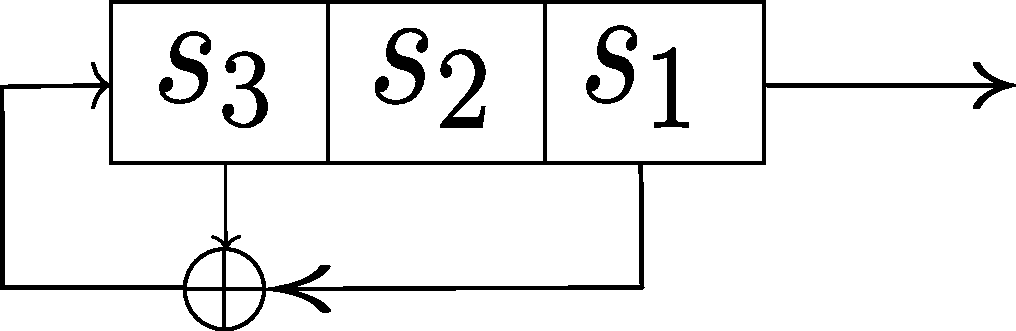
\includegraphics[scale=0.3]{imgs/lfsr1.pdf}
    }
    \caption{LFSR cu polinomul de conexiune $ C(X) = X^3 + X + 1 $}
    \label{fig:lfsr1}
  \end{figure}
\end{example}

Vom fi interesați de cazul particular din definiția următoare.

\begin{definition}\label{def:pol-prim}
  Polinomul $ C(X) $ este \emph{primitiv} dacă și numai dacă este ireductibil.
  În acest caz, vom avea $ \FF_2[X]/(C(X)) = \FF_{2^L} $, iar
  $ \FF_{2^L}^\times = \langle \theta \rangle $, grup ciclic, generat de
  o rădăcină a lui $ C $.
\end{definition}

De asemenea:
\begin{itemize}
\item dacă $ c_L = 0 $ (spunem că polinomul este \emph{singular}),
  atunci șirul devine periodic mai tîrziu;
\item dacă $ c_L = 1 $ și $ C $ este ireductibil, atunci obținem
  un șir periodic, cu perioada $ N $, care divide $ 2^L - 1 $ (va
  fi cea mai mică valoare astfel încît $ C(X) \mid 1 + X^N $;
\item dacă $ c_L = 1 $ și $ C $ este primitiv, atunci chiar $ N = 2^L - 1 $.
\end{itemize}

\begin{example}
  Dacă $ L = 4 $ și $ C = X^3 + X + 1 $ (singular) și:
  \[
    M = \begin{pmatrix}
      0 & 1 & 0 & 0 \\
      0 & 0 & 1 & 0 \\
      0 & 0 & 0 & 1 \\
      0 & 1 & 0 & 1
    \end{pmatrix}
  \]
  iar figura arată astfel:
  \[
    \xymatrix{
      s_{12} \ar[d] & s_2 \ar[d] & s_5 \ar[d] & s_6 \ar[d] & & \\
      s_9 \ar[d] & s_4 \ar[l] & s_{10} \ar[l] & s_{13} \ar[l] & & \\
      s_3 \ar[r] & s_7 \ar[r] & s_{14} \ar[ur] & s_8 \ar[r] & s_0 \\
      s_1 \ar[u] & s_{11} \ar[u] & s_{15} \ar[u] & & &
    }
  \]
\end{example}

\begin{example}
  Dacă $ C(X) = X^4 + X^3 + X^2 + X + 1 = (X + 1)(X^3 + X + 1) $,
  avem matricea:
  \[
    M = \begin{pmatrix}
      0 & 1 & 0 & 0 \\
      0 & 0 & 1 & 0 \\
      0 & 0 & 0 & 1 \\
      1 & 1 & 1 & 0
    \end{pmatrix},
  \]
  iar figura:
  \[
    \xymatrix{
      s_8 \ar[d] & s_{12} \ar[l] & s_6 \ar[l] & s_{11} \ar[l] \\
      s_1 \ar[r] & s_2 \ar[r] & s_5 \ar[ur] &
    } \quad
    \xymatrix{
      s_4 \ar[d] & s_{10} \ar[l] & s_{13} \ar[l] & s_{14} \ar[l] \\
      s_9 \ar[r] & s_3 \ar[r] & s_7 \ar[ur] &
    }
  \]
\end{example}

\begin{example}
  Pentru cazul $ C(X) = X^4 + X + 1 $, care este ireductibil și primitiv,
  avem:
  \[
    M = \begin{pmatrix}
      0 & 1 & 0 & 0 \\
      0 & 0 & 1 & 0 \\
      0 & 0 & 0 & 1 \\
      1 & 0 & 0 & 1
    \end{pmatrix}
  \]
  și se obține un ciclu de lungime 15.
\end{example}

%%% Local Variables:
%%% mode: latex
%%% TeX-master: "../criptav"
%%% End: